\documentclass[conference]{IEEEtran}
\IEEEoverridecommandlockouts
\usepackage{cite}
\usepackage{amsmath,amssymb,amsfonts}
\usepackage{algorithmic}
\usepackage{graphicx}
\usepackage{textcomp}
\usepackage{xcolor}
\usepackage{subcaption}
\usepackage{booktabs}
\usepackage{tikz}
\usetikzlibrary{positioning,arrows.meta,calc,fit,backgrounds}
\def\BibTeX{{\rm B\kern-.05em{\sc i\kern-.025em b}\kern-.08em
    T\kern-.1667em\lower.7ex\hbox{E}\kern-.125emX}}

\graphicspath{{./}}

\newcommand{\figph}[2]{%
  \IfFileExists{#2}%
    {\includegraphics[width=#1]{#2}}%
    {\fbox{\parbox[c][0.28\textwidth][c]{#1}{\centering\ttfamily\small
       [ TODO: provide figure\\ #2 ]}}}%
}

\begin{document}

\title{Museum-Guard: A Web of Things Architecture for the\\ Protection of Museum Artifacts}
\author{\IEEEauthorblockN{Simone Tassi}
\IEEEauthorblockA{\textit{Department of Computer Science and Engineering, University of Bologna, Italy} \\
simone.tassi@studio.unibo.it}
}

\maketitle

\begin{abstract}
A museum must protect its works from damage and theft, but the equipment that does this has to stay small and cheap, and it must not disturb the exhibition. This report presents \textbf{Museum-Guard}, a distributed Internet of Things system that guards a single artefact against two threats: an \textbf{impact} (a sudden mechanical shock) and a \textbf{theft} (the removal of the piece from its support). The system is built on the W3C \textbf{Web of Things} (WoT). A sensor node that speaks \textbf{CoAP} and an actuator node that speaks \textbf{HTTP} are both exposed as WoT Things, so the layers above them use one common interface and do not need to know the protocol underneath. Detection runs on the device: as soon as the firmware sees a threat, it pushes the event to its subscribers, and a visual alarm follows. Next to this security role, a closed control loop keeps the conservation lighting near a safe level, and an optional \textbf{ARIMA forecast} lets it act on changes in natural light before they happen instead of after. Every reading, event and command is stored as \textbf{timeseries} and shown on a live dashboard, while a separate consumer sends the alerts to a messaging channel. The outcome is a small system where two devices with different protocols are driven through one common model, and every layer can be seen from the same dashboard.
\end{abstract}

\begin{IEEEkeywords}
Web of Things, Internet of Things, CoAP, ESP32, anomaly detection, timeseries, adaptive lighting
\end{IEEEkeywords}

\section{Introduction}
\label{sec:introduction}

\subsection{Context: IoT and the Web of Things}
Low cost embedded devices are easy to find today, and they make it simple to monitor a physical space. A museum is a good example: its collection needs constant supervision, but the equipment that protects it must stay small, cheap and easy to place next to each exhibit. A single small node, set beside one artefact, can report on the object and on its surroundings without disturbing the visitors.

Spreading many devices like this runs into a well known problem. The Internet of Things is divided across many communication protocols, so a sensor that speaks CoAP cannot talk directly to an actuator that speaks HTTP; connecting them usually means writing dedicated code for each pair. The \textbf{Web of Things} (WoT), a W3C standard, solves this at a higher level. It describes each device with a \textbf{Thing Description}, a machine readable document that lists the device's properties, actions and events without depending on the transport protocol. Any client that can read this document can then use the device, whatever protocol carries the data.

Museum-Guard puts this idea to work in a real museum setting. It protects a single artefact from two different threats. The first, an \textbf{impact}, is a sudden mechanical shock, for example from careless handling or transport. The second, a \textbf{theft}, is the removal of the artefact from its support, which the system detects from a lasting change in its orientation. A third task is less urgent but still important for conservation: keeping the ambient light close to a level that is safe for the exhibited material.

\subsection{Project Objectives}
The project has four objectives. They also follow the structure of the rest of this report.

\begin{itemize}
\item \textbf{Protocol heterogeneous device integration:}
The first objective is to connect two devices that use different protocols and data formats: the sensing node uses CoAP, the actuation node uses HTTP. The system exposes both as uniform Web of Things resources, so a consumer works with one common model and never has to deal with the protocol underneath.

\item \textbf{Real time threat detection and response:}
Threat detection runs on the device itself, not in the cloud. The node checks its own readings and reports a problem as soon as it appears, pushing the event to its subscribers. The response is immediate too: a timed visual alarm for an impact, and a permanent one for a theft.

\item \textbf{Adaptive and predictive lighting:}
The lighting is handled by a closed loop. The system measures the ambient light and adjusts a dimmable lamp (a PWM LED in the experimental setup, it will be addressed as lamp for representation purposes) to hold it at the wanted conservation level. When enabled, an \textbf{ARIMA} forecast predicts changes in natural light, so the loop can act before they happen instead of only after.

\item \textbf{Observability and alerting:}
Finally, every reading, event and command is saved in a timeseries database and shown on a live dashboard. The events are also sent to a messaging channel, so a custodian can be notified even when far from the console.

\end{itemize}

\subsection{Document Structure}
The rest of this report is organised as follows. Section~\ref{sec:architecture} describes the architecture and the WoT interaction model. Section~\ref{sec:implementation} presents the technology stack and how each component is built. Section~\ref{sec:results} reports the evaluation.

\section{Project Architecture}
\label{sec:architecture}

Museum-Guard uses a distributed, event driven architecture, based on the Producer and Consumer roles of the Web of Things. The controller is the Producer: it owns the two Things and publishes their descriptions. The other components are Consumers: they can read those descriptions and use the system through them.

The architecture has three layers, each with its own role. At the edge are the small devices, whose firmware does the sensing, the detection and the actuation. The controller is the middle layer: it connects the devices to the abstract Things and hides the CoAP and HTTP protocols behind a single interface. At the top, the Consumers contain the application logic and never talk to the hardware directly. This separation keeps the firmware simple, keeps the protocol details inside the controller, and lets new Consumers join without changing the rest of the system.

\subsection{System Components}
The system has seven components, listed below and shown in Fig.~\ref{fig:architecture}.

\begin{itemize}
\item \textbf{ESP-SEN sensing node:}
An ESP32 board that works as a \textbf{CoAP} server. It reads an MPU-6050 accelerometer and an LDR light sensor, runs the impact and theft detection on board, and exposes the events as observable CoAP resources.

\item \textbf{ESP-ACT actuation node:}
A second ESP32 board that works as an \textbf{HTTP} server. It drives a dimmable lamp with PWM and a fixed alarm LED, and it manages the alarm timing, including the blink duration and the theft latch.

\item \textbf{WoT Controller:}
The Producer of the system. It creates and exposes the two Things over HTTP, and an adapter layer connects the two device protocols. The controller is also the only subscriber to the sensing node's observe streams, and it forwards them as Thing events.

\item \textbf{Mashup consumer:}
The main Consumer, which holds the application logic. It sets the polling interval, runs the lighting control loop, responds to threat events, and saves every reading and event in the timeseries database.

\item \textbf{Light forecast service:}
An independent \textbf{FastAPI} service that gives an ARIMA prediction of the illuminance. It helps the lighting control loop, but it is not a Thing, and the rest of the system works without it.

\item \textbf{Telegram bot consumer:}
A small Consumer that subscribes to the same threat events and sends them to a Telegram chat, as immediate alert notifications.

\item \textbf{Observability stack:}
\textbf{InfluxDB~3} stores the telemetry as timeseries, and \textbf{Grafana} shows it on a live dashboard. Together they give both a historical record and a live view of the system.

\end{itemize}

\begin{figure}[htbp]
\centering
\resizebox{\columnwidth}{!}{%
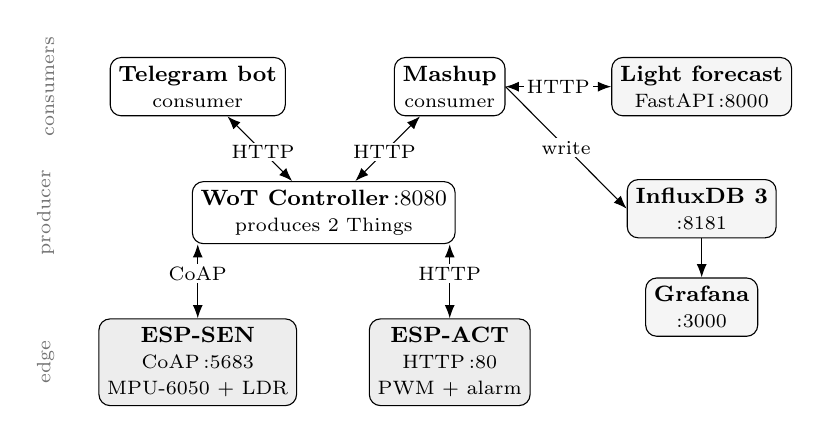
\begin{tikzpicture}[
  font=\footnotesize,
  box/.style={draw, rounded corners, align=center, inner sep=3pt, fill=white},
  dev/.style={box, fill=black!7},
  obs/.style={box, fill=black!4},
  el/.style={font=\scriptsize, fill=white, inner sep=1pt},
  lk/.style={<->, >=Latex},
]
\node[box] (tg) at (0,0) {\textbf{Telegram bot}\\{\scriptsize consumer}};
\node[box] (mashup) at (3.2,0) {\textbf{Mashup}\\{\scriptsize consumer}};
\node[obs] (fc) at (6.4,0) {\textbf{Light forecast}\\{\scriptsize FastAPI\,:8000}};
\node[obs] (influx) at (6.4,-1.55) {\textbf{InfluxDB 3}\\{\scriptsize :8181}};
\node[obs] (graf) at (6.4,-2.8) {\textbf{Grafana}\\{\scriptsize :3000}};
\node[box, minimum width=3.2cm] (ctrl) at (1.6,-1.6)
  {\textbf{WoT Controller}\,:8080\\{\scriptsize produces 2 Things}};
\node[dev] (sen) at (0,-3.5) {\textbf{ESP-SEN}\\{\scriptsize CoAP\,:5683}\\{\scriptsize MPU-6050 + LDR}};
\node[dev] (act) at (3.2,-3.5) {\textbf{ESP-ACT}\\{\scriptsize HTTP\,:80}\\{\scriptsize PWM + alarm}};
\draw[lk] (tg) -- (ctrl) node[el,pos=.55]{HTTP};
\draw[lk] (mashup) -- (ctrl) node[el,pos=.55]{HTTP};
\draw[lk] (mashup) -- (fc) node[el,pos=.5]{HTTP};
\draw[lk] (sen.north) -- (sen.north |- ctrl.south) node[el,pos=.6]{CoAP};
\draw[lk] (act.north) -- (act.north |- ctrl.south) node[el,pos=.6]{HTTP};
\draw[->,>=Latex] (mashup.east) -- (influx.west) node[el,pos=.5]{write};
\draw[->,>=Latex] (influx) -- (graf);
\node[font=\scriptsize, text=black!55, rotate=90, anchor=south] at (-1.7,0) {consumers};
\node[font=\scriptsize, text=black!55, rotate=90, anchor=south] at (-1.7,-1.6) {producer};
\node[font=\scriptsize, text=black!55, rotate=90, anchor=south] at (-1.7,-3.5) {edge};
\end{tikzpicture}%
}
\caption{High level system architecture: the WoT Producer/Consumer topology and the CoAP/HTTP protocol bindings between the controller and the two ESP32 nodes.}
\label{fig:architecture}
\end{figure}

\subsection{Thing Descriptions and Interaction Model}
The Thing Description is the contract between the Producer and the Consumers. The two descriptions are kept as plain JSON objects inside the controller's source code, in this way the exposed interface stays explicit and under version control.

A Thing offers three kinds of affordance, and Museum-Guard uses all of them: properties expose state, actions request a change of state, and events tell the Consumers that something has happened. Each kind follows a different interaction pattern. Properties such as \texttt{ambientLight} and \texttt{acceleration} are read on demand, in a request response way. The controller keeps no internal cache and reads the device only when asked, so the mashup alone decides the sampling frequency. Events such as \texttt{impactDetected} and \texttt{theftDetected}, instead, are pushed by the server to the subscribers as soon as the firmware raises them. Table~\ref{tab:things} summarises the affordances of the two Things.

\begin{table}[htbp]
\caption{WoT affordances exposed by the two Things.}
\label{tab:things}
\centering
\footnotesize
\begin{tabular}{@{}lll@{}}
\toprule
\textbf{Thing} & \textbf{Affordance} & \textbf{Kind} \\
\midrule
\texttt{museumguard-} & \texttt{ambientLight} (lux) & property (ro) \\
\texttt{sensor}       & \texttt{acceleration} (x/y/z) & property (ro) \\
& \texttt{impactThreshold} & property (rw) \\
& \texttt{theftThreshold} & property (rw) \\
& \texttt{impactDetected} & event \\
& \texttt{theftDetected} & event \\
\midrule
\texttt{museumguard-} & \texttt{variableLedIntensity} & property (ro) \\
\texttt{actuator}     & \texttt{fixedLedState} & property (ro) \\
& \texttt{setLightingIntensity} & action \\
& \texttt{triggerImpactAlarm} & action \\
& \texttt{triggerTheftAlarm} & action \\
& \texttt{resetAlarms} & action \\
\bottomrule
\end{tabular}
\end{table}

\subsection{Deployment and Information Flow}
Three information flows traverse the system. Two are event-driven, handling impact and theft detection, while the third regulates the ambient lighting. Despite their different purposes, they follow the same communication pattern: the sensing node detects a condition, the controller mediates the interaction, and a Consumer determines the appropriate response.


\textbf{Impact flow.} When ESP-SEN detects a sharp jerk along the longitudinal axis, it pushes an event to its observers with CoAP observe. The controller receives the notification and emits the \texttt{impactDetected} event of the sensor Thing. The mashup, which is subscribed to this event, saves it in the database and calls the \texttt{triggerImpactAlarm} action. The actuation node then blinks its alarm LED for twenty seconds, and times the interval by itself.

\textbf{Theft flow.} A theft is recognised from a vertical deviation that lasts, not from a single spike. ESP-SEN checks the condition over several consecutive samples before it publishes the \texttt{theftDetected} event. The mashup saves the event and calls \texttt{triggerTheftAlarm}, which keeps the alarm LED permanently on. This latched state has priority over any active impact alarm, and only an explicit \texttt{resetAlarms} action clears it.

\textbf{Lighting flow.} The lighting flow is different: it is driven by periodic polling. At each interval, the mashup reads the ambient light, optionally replaces the reading with an ARIMA forecast, and computes the intensity needed to reach the conservation target of $300$ lux. It then calls \texttt{setLightingIntensity}, and the actuation node updates the PWM duty cycle of the dimmable lamp.

This difference between the flows is intentional. Rare but time critical events are sent immediately, while the ambient light changes slowly and is sampled at a fixed interval. This design avoids unnecessary communication, but stays responsive when an immediate action is needed.

\begin{figure}[htbp]
\centering
\resizebox{\columnwidth}{!}{%
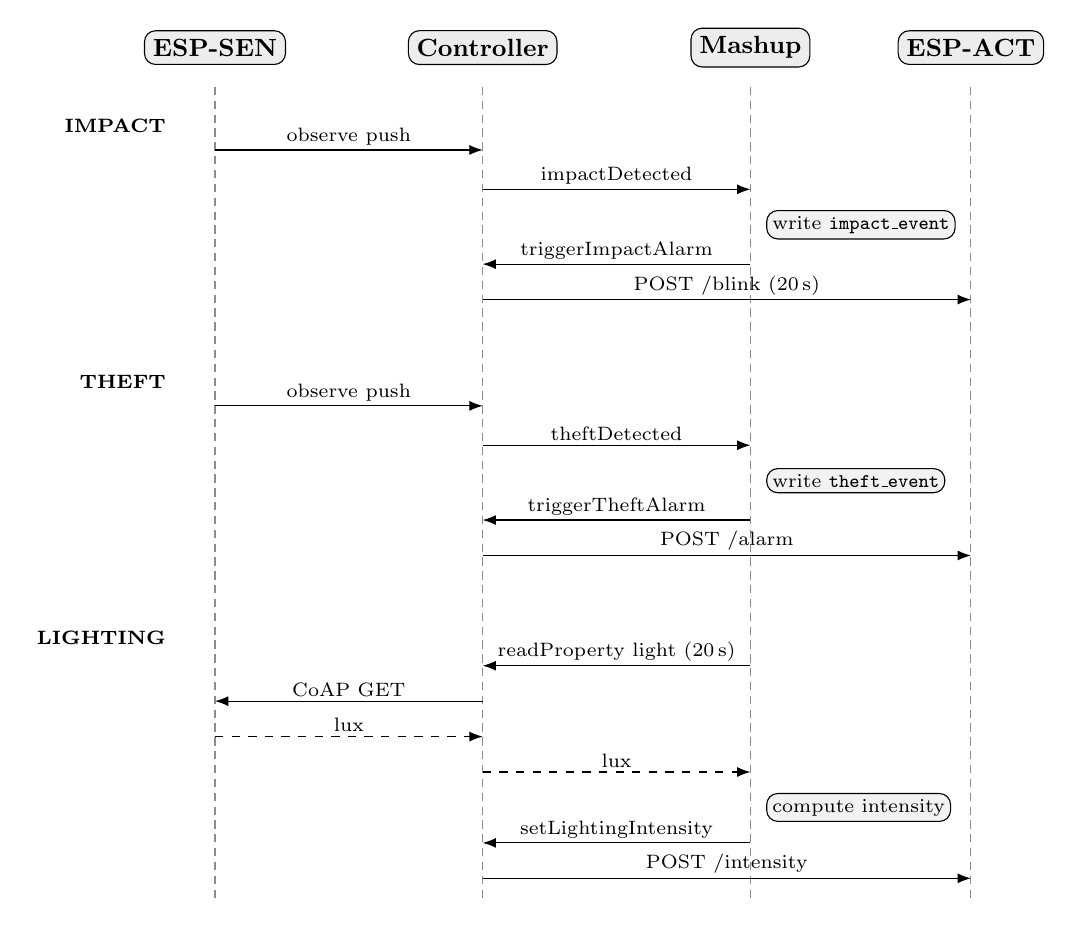
\begin{tikzpicture}[
  font=\footnotesize, >=Latex,
  head/.style={draw, rounded corners, fill=black!7, align=center, inner sep=3pt, font=\small\bfseries},
  msg/.style={->},
  ret/.style={->, dashed},
  ml/.style={font=\scriptsize, midway, above, inner sep=1.5pt},
  note/.style={font=\scriptsize, fill=black!5, draw, rounded corners, inner sep=2pt, anchor=west, xshift=2mm},
  band/.style={font=\scriptsize\bfseries, anchor=east},
]
\def\sx{0}\def\cx{3.4}\def\mx{6.8}\def\ax{9.6}
\node[head] at (\sx,0) {ESP-SEN};
\node[head] at (\cx,0) {Controller};
\node[head] at (\mx,0) {Mashup};
\node[head] at (\ax,0) {ESP-ACT};
\foreach \x in {\sx,\cx,\mx,\ax} \draw[densely dashed, black!45] (\x,-0.5) -- (\x,-10.8);
\node[band] at (-0.5,-1.0) {IMPACT};
\draw[msg] (\sx,-1.3) -- (\cx,-1.3) node[ml]{observe push};
\draw[msg] (\cx,-1.8) -- (\mx,-1.8) node[ml]{impactDetected};
\node[note] at (\mx,-2.25) {write \texttt{impact\_event}};
\draw[msg] (\mx,-2.75) -- (\cx,-2.75) node[ml]{triggerImpactAlarm};
\draw[msg] (\cx,-3.2) -- (\ax,-3.2) node[ml]{POST /blink (20\,s)};
\node[band] at (-0.5,-4.25) {THEFT};
\draw[msg] (\sx,-4.55) -- (\cx,-4.55) node[ml]{observe push};
\draw[msg] (\cx,-5.05) -- (\mx,-5.05) node[ml]{theftDetected};
\node[note] at (\mx,-5.5) {write \texttt{theft\_event}};
\draw[msg] (\mx,-6) -- (\cx,-6) node[ml]{triggerTheftAlarm};
\draw[msg] (\cx,-6.45) -- (\ax,-6.45) node[ml]{POST /alarm};
\node[band] at (-0.5,-7.5) {LIGHTING};
\draw[msg] (\mx,-7.85) -- (\cx,-7.85) node[ml]{readProperty light (20\,s)};
\draw[msg] (\cx,-8.3) -- (\sx,-8.3) node[ml]{CoAP GET};
\draw[ret] (\sx,-8.75) -- (\cx,-8.75) node[ml]{lux};
\draw[ret] (\cx,-9.2) -- (\mx,-9.2) node[ml]{lux};
\node[note] at (\mx,-9.65) {compute intensity};
\draw[msg] (\mx,-10.1) -- (\cx,-10.1) node[ml]{setLightingIntensity};
\draw[msg] (\cx,-10.55) -- (\ax,-10.55) node[ml]{POST /intensity};
\end{tikzpicture}%
}
\caption{Sequence of the three information flows (impact, theft, lighting) across the device, controller and consumer tiers.}
\label{fig:dataflow}
\end{figure}
\section{Project Implementation}
\label{sec:implementation}

\subsection{Technology Stack Overview}
The stack is made of several runtimes, each picked for its job. The small nodes run native firmware, close to the hardware, while the orchestration and application layers sit on higher level runtimes.

\begin{itemize}
    \item \textbf{Device firmware (ESP-IDF + FreeRTOS):}
    Both boards run the ESP-IDF framework on top of FreeRTOS, which gives the firmware preemptive tasks and the usual synchronisation primitives. ESP-SEN uses \textbf{libcoap} for its CoAP server, while ESP-ACT uses the HTTP server included in ESP-IDF.

    \item \textbf{Controller and consumers (Node.js / TypeScript):}
    The controller and the two consumers are written in TypeScript on Node.js. They are based on \textbf{@node-wot/core} and its \textbf{binding-http} package, the reference implementation of the Web of Things. The device adapters use the native \texttt{coap} client and \texttt{axios}, and every service logs through \texttt{pino}.

    \item \textbf{Forecasting (Python):}
    The forecasting service is a small Python application. \textbf{FastAPI} exposes the endpoint, \textbf{statsmodels} fits the ARIMA model, and \texttt{pandas} prepares the series, which is read from the database with the \texttt{influxdb3-python} client.

    \item \textbf{Infrastructure:}
    \textbf{InfluxDB~3} and \textbf{Grafana} provide storage and visualisation. Both are defined in \textbf{Docker Compose}, so the stack starts with a single command, and its configuration is already in place.
\end{itemize}

\subsection{ESP-SEN Sensor Firmware}

\subsubsection{Hardware and Sampling}
The sensing node has two transducers. An MPU-6050 accelerometer is read over I2C at $400$\,kHz; the data and clock lines are on GPIO21 and GPIO38, and the full scale range is $\pm 8$\,g. An LDR forms a voltage divider with a $10$\,k$\Omega$ resistor. Its midpoint is read on ADC channel~6 (GPIO7), and the illuminance comes from the inverse relation $\mathit{lux} = 500000 / R_{\mathrm{LDR}}$. The accelerometer is mounted in a rotated position, so the firmware normalizes its readings at the driver boundary into a standard body frame where $z$ is vertical (gravity) and $x$ longitudinal; the rest of the system then uses the usual convention. Figure~\ref{fig:circuit} shows the wiring of both nodes on a shared breadboard.

A single FreeRTOS task manages the acquisition: it reads the accelerometer every $50$\,ms (a rate of $20$\,Hz), and the slower light sensor once per second. A mutex protects the shared sensor state from concurrent access, and a queue passes the detected events to the network task, so detection and notification never block each other.

\begin{figure}[htbp]
    \centering
    \figph{0.45\textwidth}{circuit.png}
    \caption{Wiring of both nodes on a shared breadboard: ESP-SEN with the MPU-6050 accelerometer (I2C, GPIO21/38) and the LDR (ADC, GPIO7), and ESP-ACT with the PWM lamp (GPIO5) and the fixed alarm LED (GPIO6).}
    \label{fig:circuit}
\end{figure}

\subsubsection{Impact and Theft Detection}
Both threats are recognised on the node, from the same accelerometer stream. The two tests look for different things.

An impact is a short, strong movement. The firmware follows the jerk along the longitudinal axis, that is the difference between two consecutive readings, $|a_x[n] - a_x[n-1]|$. When this value goes above the impact threshold ($20$\,m/s\textsuperscript{2} by default) the firmware raises an event. A one second cooldown then blocks further impacts, so a single shock is reported once and not as a burst.

A theft is the opposite: the firmware watches the vertical axis and measures its deviation from gravity, $|a_z - 9.80665|$. The deviation must stay above the theft threshold ($4$\,m/s\textsuperscript{2} by default) for at least five consecutive samples (a quarter of a second), before the event fires. A three second cooldown follows.

The firmware ships with default thresholds that can be overridden at runtime. Both are exposed as writable Thing properties and can be changed through the \texttt{config/impact-threshold} and \texttt{config/theft-threshold} CoAP resources, so an operator can adjust the sensitivity without reflashing the board.

\subsubsection{CoAP Server and Observe}
The node exposes its data through a CoAP server on UDP port~$5683$. Table~\ref{tab:coap} lists the resources. The two \texttt{sensor/*} resources return the latest readings on request, and the two \texttt{config/*} resources read and write the detection thresholds.

The event resources work differently. A client subscribes to \texttt{events/impact} or \texttt{events/theft} with the observe option of CoAP. When the detection logic raises an event, the firmware calls \texttt{coap\_resource\_notify\_observers}, and libcoap pushes the new value to every subscriber. This is the standard observe mechanism of the protocol, and the controller no longer needs to poll for anomalies. Each reading and event has an ISO-8601 timestamp, taken from an SNTP client that is synchronised at start up, so the records stay aligned with the rest of the system.

\begin{table}[htbp]
\caption{ESP-SEN CoAP resources (UDP :5683).}
\label{tab:coap}
\centering
\footnotesize
\begin{tabular}{@{}lll@{}}
\toprule
\textbf{Resource} & \textbf{Method} & \textbf{Observable} \\
\midrule
\texttt{sensor/light} & GET & no \\
\texttt{sensor/acceleration} & GET & no \\
\texttt{events/impact} & GET & yes \\
\texttt{events/theft} & GET & yes \\
\texttt{config/impact-threshold} & GET/PUT & no \\
\texttt{config/theft-threshold} & GET/PUT & no \\
\bottomrule
\end{tabular}
\end{table}

\subsection{ESP-ACT Actuator Firmware}

\subsubsection{LED Drivers}
The actuation node controls two light sources, both managed by a single FreeRTOS task that receives commands through a queue. The artwork lamp is on GPIO5 and is driven by the LEDC peripheral with a PWM signal at $5$\,kHz and $13$-bit resolution. Its brightness is set on request: a set intensity command carries a percentage, and the task maps it linearly onto the duty cycle, from off at 0 to full brightness at 100. The alarm indicator is a second LED on GPIO6, used as a simple on/off output, because it only needs to be on or off.

\subsubsection{Alarm Handling}
The same task also handles the alarm, with three more commands: blink, alarm, and reset. Because the timing is managed by the device, the node alone decides how its alarm behaves.

An impact starts a twenty second blink: the LED toggles every $250$\,ms, and the task switches it off when the interval ends. A theft instead keeps the LED permanently on, and this state has priority: while it is active, a blink request is ignored, and only a reset clears it. The current state is exposed as \texttt{fixedLedState}, which is \texttt{off}, \texttt{blinking} or \texttt{on}, and the controller just reads it back.

\subsubsection{HTTP API}
The node is reached through a small HTTP API on port~$80$, shown in Table~\ref{tab:http}. A single \texttt{GET} returns the current intensity and alarm state, and four \texttt{POST} endpoints send the commands. Each handler validates the request, puts a command on the queue, and answers right away: a successful command returns $204$ No~Content, a malformed body returns $400$, and a queue failure returns $500$. The control task then does the work asynchronously, so the server stays responsive even while an alarm is running.

\begin{table}[htbp]
\caption{ESP-ACT HTTP API (TCP :80).}
\label{tab:http}
\centering
\footnotesize
\begin{tabular}{@{}lll@{}}
\toprule
\textbf{Method} & \textbf{Endpoint} & \textbf{Effect} \\
\midrule
GET  & \texttt{/actuator/state} & read intensity + LED state \\
POST & \texttt{/actuator/intensity} & set PWM intensity (0--100) \\
POST & \texttt{/actuator/blink} & start 20\,s impact blink \\
POST & \texttt{/actuator/alarm} & latch theft alarm on \\
POST & \texttt{/actuator/reset} & clear all alarms \\
\bottomrule
\end{tabular}
\end{table}

\subsection{WoT Controller}

\subsubsection{Thing Production and Exposure}
The controller is based on a node-wot Servient with an HTTP server binding. At start up it produces each Thing from its description with \texttt{wot.produce}, and then attaches the handlers that define the behaviour of the affordances. Property reads and writes are connected to the adapter layer, and so are the action handlers, so an interaction on a Thing becomes a request to the matching device. When the handlers are ready, \texttt{thing.expose} publishes both descriptions over HTTP on port~$8080$, where any Consumer can read them. This whole sequence is managed in \texttt{index.ts}, which also adds a \texttt{SIGINT} handler, so the observe streams and the server are closed cleanly on shutdown.

\subsubsection{Adapter Layer}
Between the abstract Things and the physical devices there is an adapter layer that hides the two transport protocols. The sensor adapter is a native CoAP client. It reads the light and the acceleration, writes the detection thresholds with CoAP PUT, and keeps the observe streams through which the events arrive. The actuator adapter is an HTTP client based on \texttt{axios}, and it also validates the input before it sends a request. Both adapters log their errors with \texttt{pino} and then rethrow them, so a failure can reach the Thing handler that started the operation.

\subsubsection{Event Bridging}
Events pass from CoAP to the Web of Things in a single place. At start up the controller subscribes once to the sensor's \texttt{events/impact} and \texttt{events/theft} resources. When a notification arrives, the controller re emits it as the matching Thing event, \texttt{impactDetected} or \texttt{theftDetected}, which the consumers receive through their normal event subscriptions. The two observe streams stay open for the whole life of the process and are cancelled on shutdown, so the controller never creates duplicate subscriptions.

\subsection{Mashup Consumer and Control Logic}

\subsubsection{Stateful Consumer and Poll Loop}
The mashup starts by consuming the two Things it will drive. Its \texttt{consumer} module is a stateful singleton: a single call to \texttt{initConsumer} fetches both descriptions from the controller and consumes them, and then \texttt{getSensor} and \texttt{getActuator} return the \texttt{ConsumedThing} handles to the rest of the application. This central state makes sure that every part of the mashup uses the same proxies, and that no Thing is consumed twice.

Periodic data comes from a poll loop, whose period is set by \texttt{POLLING\_MS} (twenty seconds by default). On each tick the loop reads the ambient light, the acceleration and the actuator's LED state, and writes each value to the database as it arrives. The three steps are independent: if one read fails, the loop logs the error and continues, so a single unreachable device does not stop the cycle. Because the controller keeps no internal copy of the sensor data, this loop sets the sampling rate of the whole system.

\subsubsection{Adaptive and Predictive Lighting}
The same loop also handles the lighting control loop. From the measured illuminance, the mashup computes the intensity needed to reach the conservation target, the constant \texttt{TARGET\_LUX}, fixed at $300$ lux. The intensity is the part of the target that is still missing, written as a percentage and clamped to the valid range,
\[
  \text{intensity} = \mathrm{clamp}\!\left(0,\;100,\;\frac{L_{\mathrm{target}} - L}{L_{\mathrm{target}}}\times 100\right),
\]
where $L$ is the control illuminance and $L_{\mathrm{target}}$ the target. For example, in a dark room the lamp goes to full brightness. The result is sent to the actuator with the \texttt{setLightingIntensity} action.

Two details refine this behaviour. First, the control is disabled while an alarm is blinking or latched, so the lamp is never changed while it signals a threat. Second, when forecasting is enabled, $L$ is the value predicted by the forecast service, not the current reading, so the system can anticipate a change in light instead of following it late. If the forecast is not available, the loop uses the latest measurement and continues without interruption.

\subsubsection{Event Handling}
Next to the poll loop, the mashup also reacts to the two threat events. At start up it calls \texttt{subscribeEvent} on \texttt{impactDetected} and \texttt{theftDetected}. Each handler does two things in order: it saves the event in the database, and it calls the matching alarm action on the actuator, \texttt{triggerImpactAlarm} or \texttt{triggerTheftAlarm}.

\subsection{Light Forecasting Service}
The mashup uses the forecasting service only when predictive lighting is enabled. It is a small FastAPI application with a single endpoint, \texttt{GET /forecast}, whose \texttt{horizon\_s} parameter sets how far ahead the prediction goes.

A request starts a short pipeline. The service reads the last 15 minutes of the \texttt{ambient\_light} measurement from the database and resamples the readings onto a regular twenty second grid, equal to the mashup's default polling period. Then it finds the differencing degree $d$ needed for stationarity with the augmented Dickey-Fuller test, up to a maximum of two (a real series almost never needs more and over-differencing would add false structure) and fits an $\mathrm{ARIMA}(1, d, 1)$ model with statsmodels. Only the differencing degree is taken from the data. The other two orders are fixed at one on purpose: the histories are short and change slowly, and the forecast reaches only a few steps ahead, so searching for the best orders at every request would overfit and could give unstable fits. One autoregressive term already captures how the light persists from one reading to the next, and one moving average term absorbs a single noisy sample. The fitted model is extended over the requested horizon, and the predicted illuminance is returned to the caller.

The service also handles the cases where a forecast would be meaningless: if the recent data is missing, too short or constant, or if the fit fails, the service drops the model and returns the last observed value, and it marks the response with a fallback flag. The mashup uses this value like any other forecast, so the lighting loop keeps working even when a real prediction is not available.

\subsection{Telegram Bot Alerting Service}
The alerting service sends threat notifications outside the dashboard. It is a second, minimal Web of Things consumer, independent of the mashup. Like the mashup, it consumes the sensor Thing and subscribes to \texttt{impactDetected} and \texttt{theftDetected}, but it does not take part in storage or control.

When an event arrives, the service builds a short message with the value and the timestamp of the event, and sends it to the Telegram \texttt{sendMessage} Bot API as HTML. Running this path as a separate consumer keeps it independent from the mashup, and shows how new consumers can connect to the same Things without any change to the producer.

\subsection{Observability and Orchestration}

\subsubsection{Timeseries Schema}
All the telemetry of the system goes to a single InfluxDB~3 database, \texttt{museumguard}, written by the mashup. Seven measurements cover the full state of the installation, listed in Table~\ref{tab:influx}. Three of them record what the sensor observes: the ambient light, its forecast and the acceleration components. Two more record the impact and theft events. The last two describe the actuator: the lamp intensity and the alarm LED state. Every point has a \texttt{node} tag with the name of the device it came from, so sensor and actuator data can be separated in a query.

\begin{table}[htbp]
\caption{InfluxDB measurements written by the mashup.}
\label{tab:influx}
\centering
\footnotesize
\begin{tabular}{@{}lll@{}}
\toprule
\textbf{Measurement} & \textbf{Fields} & \textbf{Tag} \\
\midrule
\texttt{ambient\_light} & \texttt{lux} & \texttt{node=esp-sen} \\
\texttt{ambient\_light\_forecast} & \texttt{lux} & \texttt{node=esp-sen} \\
\texttt{acceleration} & \texttt{x,y,z} & \texttt{node=esp-sen} \\
\texttt{impact\_event} & \texttt{value} & \texttt{node=esp-sen} \\
\texttt{theft\_event} & \texttt{value} & \texttt{node=esp-sen} \\
\texttt{lighting\_intensity} & \texttt{intensity} & \texttt{node=esp-act} \\
\texttt{fixed\_led\_state} & \texttt{state} & \texttt{node=esp-act} \\
\bottomrule
\end{tabular}
\end{table}

\subsubsection{Grafana Provisioning and Docker}
Storage and visualisation are deployed together with Docker Compose. The compose file defines two services: InfluxDB~3, on port~$8181$ with a file based object store and an administration token given as a secret, and Grafana on port~$3000$. Grafana is configured from version controlled files, not by hand. A datasource connects it to the database, and a dashboard, \emph{MuseumGuard Overview}, is loaded from \texttt{grafana/dashboards/museumguard.json}. Its panels, shown in Fig.~\ref{fig:dashboard}, present the light, the acceleration, the events and the alarm state together, including a direct comparison between the measured illuminance and its forecast.

\begin{figure*}[htbp]
    \centering
    \figph{\linewidth}{dashboard.png}
    \caption{The Grafana ``MuseumGuard Overview'' dashboard, demonstrating the full telemetry pipeline: ambient light and lamp intensity, the security event log, and the alarm state timeline.}
    \label{fig:dashboard}
\end{figure*}


\section{Results}
\label{sec:results}

The complete system was assembled on the two ESP32 boards and the PC side services, to check that the components work together as intended. The evaluation is partly quantitative, with the detection stage measured through controlled trials and the light forecast measured against a naive baseline, and partly qualitative, describing the behaviour of actuation and lighting, with the Grafana dashboard giving a continuous record during the tests.

\subsection{Functional Behaviour}
Detection and resposne worked as designed. A sharp knock on the support reliably produced an \texttt{impactDetected} event, which passed through the controller to the mashup and turned on the blinking alarm for twenty seconds, before it cleared itself. Lifting or tilting the artefact for more than a fraction of a second produced a \texttt{theftDetected} event and latched the alarm on until a reset. When a theft arrived during an impact blink, the latch correctly took priority. Changing the thresholds at runtime, through the two \texttt{config} resources, changed the sensitivity at once and without reflashing, so both behaviours were easy to trigger and to tune. At the same time, the adaptive lighting kept the lamp near the target level: it raised the intensity as the room got darker, and lowered it as the ambient light came back. Each event also reached the Telegram chat almost immediately, which confirms that a second consumer can observe the same Things without any change to the producer.

\subsection{Detection Accuracy}
\label{sec:detection}
To measure the detection stage, each threat was tested under controlled trials at three thresholds around the default. For each threshold the artefact received $20$ deliberate threats and $20$ "benign" actions of the kind normal handling produces, such as taps on the support, people passing by, and light contact below the intended sensitivity. Each benign action counts as a negative case, so the True Negative count is well defined and the false alarm rate (FPR) has a clear denominator instead of being measured over time. The threats were counted by hand, and the raised events were checked against the firmware log, while the thresholds were changed between blocks at runtime through the two \texttt{config} resources, so the whole process needed no reflashing.

\begin{table}[htbp]
\caption{Detection sweep: $20$ deliberate threats and $20$ benign opportunities per configuration. Threshold in m/s\textsuperscript{2}; the default of each threat is highlighted.}
\label{tab:detection}
\centering
\footnotesize
\begin{tabular}{@{}llrrrrrr@{}}
\toprule
\textbf{Threat} & \textbf{Thr.} & \textbf{TP} & \textbf{FN} & \textbf{FP} & \textbf{TN} & \textbf{TPR} & \textbf{FPR} \\
\midrule
Impact & $10$ & $20$ & $0$ & $5$ & $15$ & $1.00$ & $0.25$ \\
\textbf{Impact} & \textbf{20} & \textbf{19} & \textbf{1} & \textbf{2} & \textbf{18} & \textbf{0.95} & \textbf{0.10} \\
Impact & $30$ & $8$  & $12$ & $0$ & $20$ & $0.40$ & $0.00$ \\
\midrule
Theft & $2$ & $19$ & $1$ & $7$ & $13$ & $0.95$ & $0.35$ \\
\textbf{Theft} & \textbf{4} & \textbf{18} & \textbf{2} & \textbf{0} & \textbf{20} & \textbf{0.90} & \textbf{0.00} \\
Theft & $6$ & $4$  & $16$ & $0$ & $20$ & $0.20$ & $0.00$ \\
\bottomrule
\end{tabular}
\end{table}

Table~\ref{tab:detection} gives the confusion counts with the detection rate ($\mathrm{TPR}=\mathrm{TP}/(\mathrm{TP}+\mathrm{FN})$) and the false alarm rate ($\mathrm{FPR}=\mathrm{FP}/(\mathrm{FP}+\mathrm{TN})$), and Figure~\ref{fig:detection} plots the two against the threshold. Both detectors show the same trade off: as the threshold rises the false alarms fall to zero, but past a point the detection rate drops sharply, because a too high threshold stops seeing the threat. The default threshold is chosen where detection is still high and the false alarms are low, trying to find the best trade off.

\begin{figure}[htbp]
    \centering
    \figph{\linewidth}{detection_accuracy.png}
    \caption{Detection rate (TPR) and false alarm rate (FPR) against the detection threshold, for impact (left) and theft (right).}
    \label{fig:detection}
\end{figure}

For impact the default is $20$\,m/s\textsuperscript{2}. The sensitive setting of $10$ catches every knock but raises five false alarms, while the high setting of $30$ removes the false alarms only by missing more than half of the real impacts, its detection falling to $0.40$. The default sits between the two, keeping detection at $0.95$ and cutting the false alarms from five to two. Unlike the theft default, it does not remove them all: raising the threshold to $30$ would clear the last false alarms but lose most of the impacts, and a short blinking alarm is much easier to accept than a permanent theft latch, so a couple of unintended blinks are a fair price for catching almost every real impact.

For theft the default is $4$\,m/s\textsuperscript{2}. The sensitive setting of $2$ catches almost every lift but fires on more than a third of the benign actions, instead, the high setting of $6$ waits so long that it misses four thefts out of five. The default catches $18$ thefts out of $20$ with no false alarm, which is what a permanent alarm needs.

\subsection{Resource Footprint}
\label{sec:footprint}
A second measurement looks at what the two nodes cost in memory, since the premise of the system is that each node stays small and cheap. Two observations matter (reported in Table~\ref{tab:footprint}): 
\begin{itemize}
    \item \textit{static footprint}: how much flash and RAM the firmware reserves when it is linked, from \texttt{idf.py size} 
    \item \textit{free heap}: how much RAM is still available at runtime once WiFi and the CoAP or HTTP stack are running, taken from a log line printed at the end of start up (removed in the final implementation) 
\end{itemize}

\begin{table}[htbp]
\caption{Memory footprint of the two nodes}
\label{tab:footprint}
\centering
\footnotesize
\begin{tabular}{@{}lrrr@{}}
\toprule
\textbf{Node} & \textbf{Flash} & \textbf{Static RAM} & \textbf{Free heap} \\
\midrule
\texttt{esp-sen} & $960$\,KB & $50$\,KB & $233$\,KB \\
\texttt{esp-act} & $840$\,KB & $36$\,KB & $258$\,KB \\
\bottomrule
\end{tabular}
\end{table}

The firmware is small on both counts. The image is under $1$\,MB of flash on a module that carries $4$\,MB, about a quarter of it, and the statically reserved data RAM is only a few tens of kilobytes. At runtime, once the network stacks are up, each node still has more than $230$\,KB of heap free, out of the roughly $320$\,KB of internal RAM. ESP-ACT is a little lighter than ESP-SEN, because it uses the built in HTTP server instead of the heavier \textbf{libcoap} stack.

\subsection{Predictive Lighting Evaluation}
\label{sec:forecast}
When forecasting is enabled, the mashup drives the lamp from the predicted illuminance instead of the latest reading, so it can anticipate a change in light rather than react to it late. The forecast was evaluated in two complementary ways: on real data collected via the experimental setup, and on a synthetic light signal that changes the way natural light would. In both cases the ARIMA prediction is compared with a naive \emph{persistence} baseline, which simply assumes the next value will equal the last one. This baseline matches what the system itself does when the forecast is off or falls back, since both drive the lamp from the last observed reading, so the comparison measures exactly the benefit of the forecast over the system's own non predictive behaviour.

The experimental test is the honest starting point, but also the least favourable. Over thirty minutes of collection the light in the room stayed almost constant, so there was very little to predict. On the $84$ forecasts produced in that window the ARIMA model and the persistence baseline both reached a mean absolute error of about $1.2$ lux, which is at the level of the sensor noise, and the model fell back to the last reading on 1/10 of the samples. The two are effectively tied ($1.11$ against $1.20$ lux), and the small gap between them is well inside the noise range. This is exactly the expected outcome: when the signal carries no real variation, the forecast can neither help nor harm, and the only useful conclusion is that the whole pipeline runs correctly from end to end.

To see what the model does when the light actually moves, it was run, with the same code and the same $60$ second horizon, on a synthetic curve. The prediction is checked with progressive validation: at each step the model forecasts one horizon ahead from the data available so far, and the prediction is compared with the value that truly follows. Table~\ref{tab:forecast-eval} reports the error for curves that change at different speeds. When the light varies slowly, the model and the baseline are close, because over one minute "assume no change" is almost right. As the light changes faster within the horizon, the persistence error grows while the model keeps following the trend, so ARIMA becomes better, down to about $60\%$ less error on the fastest curve. This signal is synthetic and only illustrates the model's behaviour, it is not a measurement of the real room.

\begin{table}[htbp]
\caption{Forecast error (mean absolute error, in lux) on synthetic daylight signals that change at different speeds, over a $60$ second horizon, against a naive persistence baseline. The model's advantage grows as the light changes faster.}
\label{tab:forecast-eval}
\centering
\footnotesize
\begin{tabular}{@{}lrrr@{}}
\toprule
\textbf{Light change} & \textbf{ARIMA} & \textbf{Persistence} & \textbf{Improvement} \\
\midrule
Slow ($3$\,h cycle)   & $4.55$ & $4.64$  & $2\%$  \\
Moderate ($90$\,min)  & $5.25$ & $7.00$  & $25\%$ \\
Fast ($45$\,min)      & $6.66$ & $13.07$ & $49\%$ \\
Very fast ($30$\,min) & $7.64$ & $18.89$ & $60\%$ \\
\bottomrule
\end{tabular}
\end{table}

Taken together, the two tests give a fair picture. On the static setup the forecast is correct but idle, and it offers a real advantage only when the ambient light moves appreciably during the forecast horizon. In every case the lamp keeps working: when a good fit is not possible the service falls back to the last reading and the loop returns to normal reactive control, and the only thing lost is the anticipation.

\subsection{Conclusions}
Together, these results show that the Web of Things abstraction works well in practice. Two devices with different protocols were unified behind uniform Things, controlled by independent consumers, and observed on a single dashboard, and no component needed to know how the others were built. The result is a small but complete artefact protection system: every layer, from the two nodes to the dashboard, can be seen and extended on its own, without touching the others.

\section*{Use of AI Assistance}
An AI assistant (Anthropic's Claude) was used in a supporting role during development, limited to these tasks: writing the \LaTeX{} tables in this report from the project's own definitions, namely the WoT affordances of the two Things, the ESP-SEN CoAP resources, the ESP-ACT HTTP endpoints and the InfluxDB measurement schema; creating the Grafana provisioning files for the Docker Compose stack, derived from a configuration first set up by hand in the Grafana interface; generating the \texttt{README} files from the existing codebase; adding logging statements to the code to support live testing and debugging; rephrasing some sentences of this report for clarity, while keeping the intended meaning; and guiding the evaluation of the ARIMA forecast on synthetic light data, used to show how the model behaves when the ambient light varies. The design choices, the system architecture, the detection algorithms and the interpretation of the results were done independently, and every AI-assisted file was reviewed and checked before inclusion.

\end{document}
